\documentclass[UTF8, 12pt]{article}

% PACKAGES
\usepackage{geometry}
\usepackage{graphicx}
\usepackage{setspace}
\usepackage{indentfirst}
\usepackage{hyperref}
\usepackage{amsmath}
\usepackage{csvsimple}
\usepackage[T1]{fontenc}
\usepackage[nottoc,notlot,notlof]{tocbibind}
\usepackage[style=ieee,sorting=none,backend=biber]{biblatex}

% DOCUMENT SETTINGS
% PAPER SETTINGS
\geometry{letterpaper,
          left=1in,
          right=1in,
          top=1in,
          bottom=1in}

% IMAGE DIRECTORY
\graphicspath{{images/}}

% OTHER SETTINGS
\renewcommand*\contentsname{Table of Contents} % change table of contents name
\renewcommand{\thefigure}{\Roman{figure}}
\addbibresource{refs.bib}

% TITLE DEFINITIONS
\title{Project Lab 2\\\large Final Report}
\author{Dirk Thieme\\R11636727\\Texas Tech University}
\date{December 2022}

% MAIN DOCUMENT
\begin{document}
\maketitle
\pagenumbering{gobble}
\newpage
\pagenumbering{arabic}
% \spacing{1.25}
\spacing{2}

% ABSTRACT
\begin{abstract}
    This paper describes the final state of the Automated Recorder Project. While the requirements of the project will be discussed more in further sections, the general goal is to automate the playing of a recorder using a Raspberry Pi, which will be able to play any song as given to it through a flash drive. The device can also be controlled using an electric piano, where one can play the recorder using the keys. This project is being developed by Dirk Thieme, Mason Hadley, Jake Kiedasch, and Mariano Arce.
\end{abstract}

\newpage
\tableofcontents

\newpage
\listoffigures

% \newpage
% \listoftables

\newpage
\section{Introduction}
    The original premise of the Automated Recorder Project is to play a grade school recorder using a Raspberry Pi. The recorder should be able to play eight notes, and would be able to play a select number of songs chosen by the instructor of the course and a local area elementary school teacher. The recorder apparatus should be able to play in front of an elementary school class.

    While the premise of the project was enough of a challenge, this project aims to go above and beyond the original scope by allowing the recorder to play all 27 notes within its capability and by allowing the user to dynamically chose the desired song to play with an MP3 file. To allow the recorder to play all notes, certain holes must only be covered halfway, a technique known as leaking and pinching \cite{rec_wiki}. To be able to play any MP3 file provided, the software will be able to process the song on demand and convert the sound wave into a collection of frequencies which correspond to notes. These notes will be automatically converted into notes that the recorder can play. The recorder will also be able to use an electric piano as a human interface to play songs manually.

    The brain of the apparatus is the Raspberry Pi 4B (furthermore Pi), a single-board computer which executes the code and controls the hardware. The Pi is powered using a quad core 64-bit ARM-Cortex A72 running at 1.5GHz \cite{ras_pi} which brings enough power to the table in order to complete the challenging digital signal processing required. The GPIO pins are also utilized to be able to control the hardware which actuates the recorder.

    The recorder is physically controlled through the use of six solenoids, three servo motors, and three compounded fans. Five of the solenoids cover and uncover the main holes, and three of the servos perform the pinching of the holes which require multiple positions. The one other solenoid opens and closes the main labium, which stops the recorder from playing to play rests. The solenoids require 12V power, while the servos and Pi require 5V power. The Pi only outputs 5V at 16mA on the GPIO pins \cite{ras_pi}, therefore a circuit has been designed in order to be able to actuate the solenoids while not burning out the GPIO pins. To power the entire setup, a 12V, 150W power supply will be able to accept AC wall power, which it can then send to a custom made power distribution PCB, which incorporates a 12V-5V buck converter and the various high power outputs, along with the solenoid circuits. The piano used to play the device is the AKAI MPK Mini MK3, a MIDI controller built-in to a 25 key keyboard, which allows the user to play songs. The piano can sweep between 10 octaves, however this device only uses about 2 \cite{piano}. The integrated USB port is plugged into the Pi and is integrated into the Python code so it can use the recorder.

    While the structure of the software is rather simple, the implementation is exceedingly complex, and requires immense amounts of research and assistance to complete. The software is controlled by the user using a GUI written using the TKinter library, where there are three tabs. The first tab is a list of songs which are built-in to the device, and one clicks on one and it plays. The second tab allows the user to ingest an MP3 file, then convert it into a WAV file. The WAV file bytestream is parsed into its proper values, then its time-domain signal is broken up into bins which are individually processed using a Fast Fourier Transform into their frequency-domain counterpart. The transform is not performed on the Pi, as the CPU would take to long, so it is sent over the Internet to a server which uses its actual full-size CPU to calculate the answer.The magnitudes of each bin are then calculated, which reveal the peak frequency of the bin, corresponding to the note at that time period. These notes are then converted into their recorder playable counterparts, which will then be played for the correct amount of time. The third tab allows the user to play the piano.

\newpage
\section{Body}
    The final state of this project is comprised of the the Software and the Hardware. The Softwre is a Python codebase which consists of the GUI and the three methods of interaction, the Custom Songs, the Hardcoded Songs, and the Piano Input. The Hardware consists of the recorder itself, the control devices, the air production, the piano input, and the Pi which runs the whole thing.

\subsection{Software}
\subsubsection{Flow of Control Chart}
    \begin{figure}[h]
        \centering
        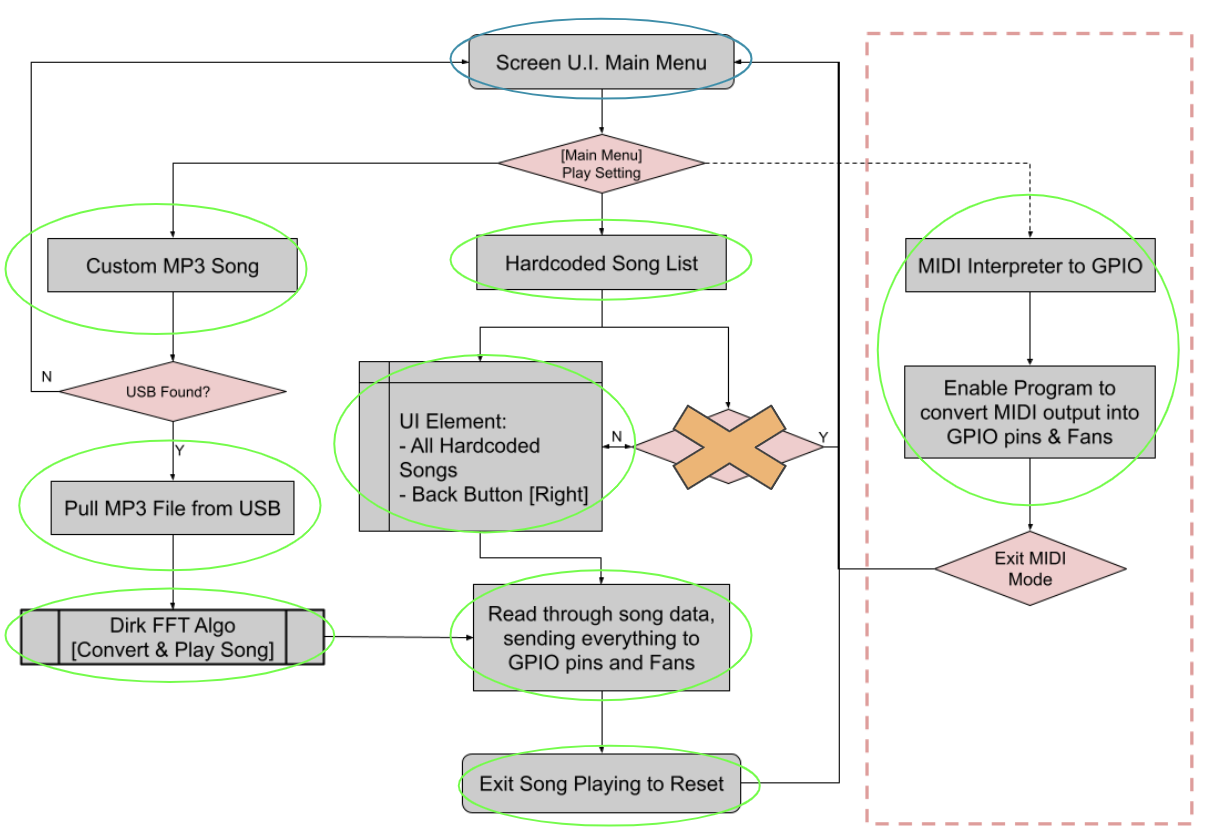
\includegraphics[width=0.75\textwidth]{flowchart}
        \caption{Main Software Flowchart}
        \label{fc}
    \end{figure}
    As shown in Figure \ref{fc}, this flowchart is the path that the software takes to complete its tasks. The screen is a basic 7-inch touchscreen, and the code just automatically opens up upon startup of the Pi. 

\subsubsection{GUI Code}
    As the touchscreen needs to be used to keep the interface compact and efficient, the GUI must be easy for fingers to touch and control, otherwise the interface would be unsatisfactory to use. The code itself is broken up into a separate class which makes it easy to edit and update accordingly. TKinter is a GUI library which breaks up the interface into different parts, the root, which contains the main window, the notebook, which is what contains the individual frames. The frames contain each interactive element, like a folder contains a file. The root is configured to popup in full screen and to accept the notebook. The notebook is configured to have three tabs which each have a single frame containing the three main aspects of the code. This is shown in Figure \ref{gui_fig}.
    \begin{figure}[h]
        \centering
        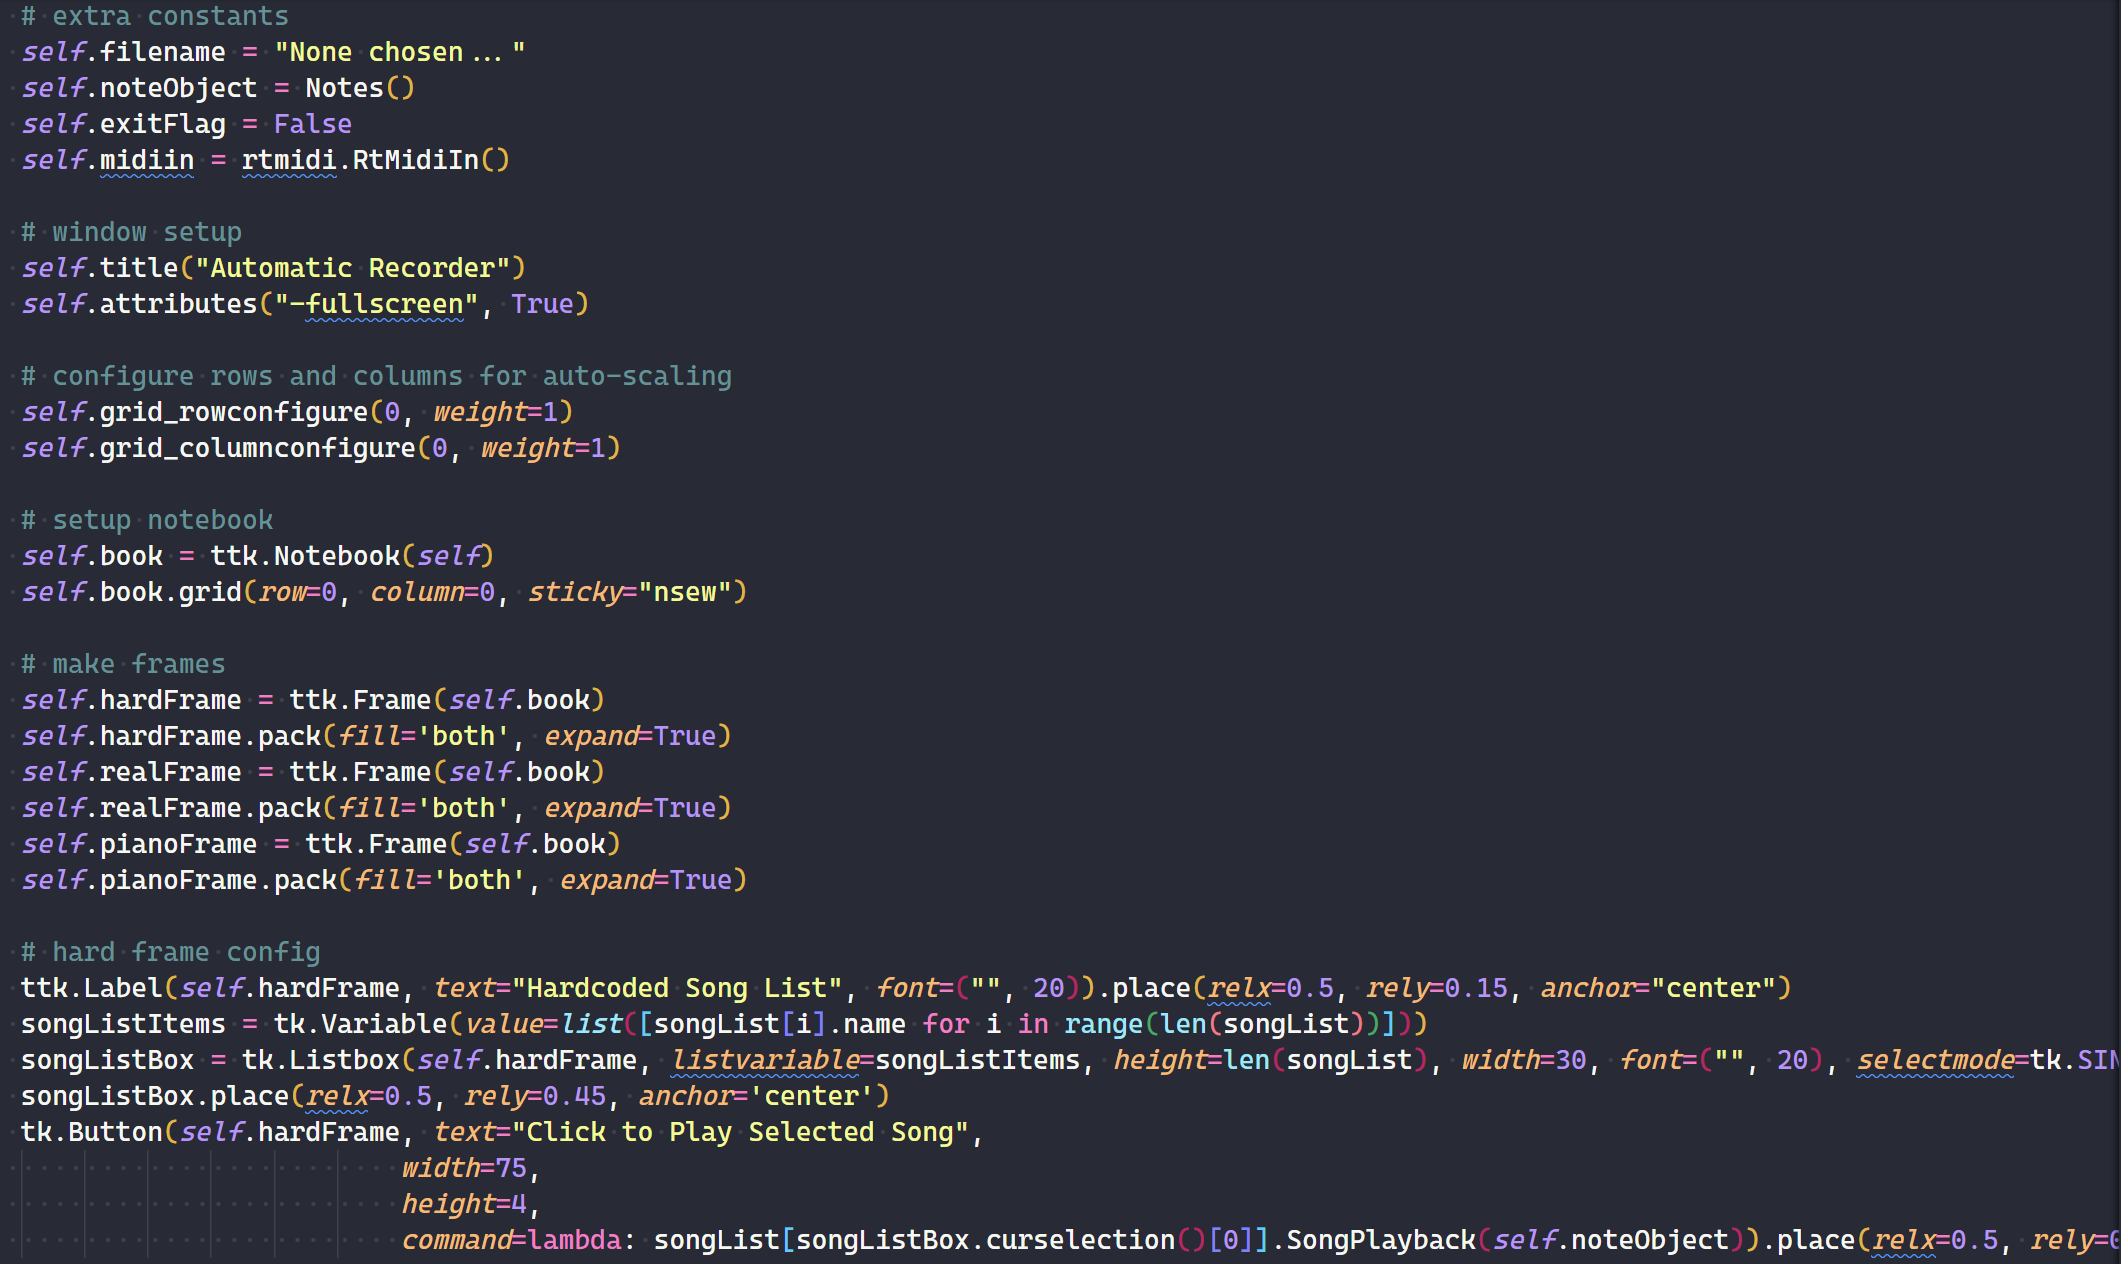
\includegraphics[width=0.75\textwidth]{gui_example}
        \caption{GUI Setup Code}
        \label{gui_fig}
    \end{figure}

\subsubsection{Notes and Fan Control}
    A class is setup which is used to control the GPIO pin outputs, including the PWM signals that control the fan and the servos, and the standard on/off signals which control the solenoids. At every startup of the code, the GPIO pins are initialized and turned off to make sure the solenoids are inactive when waiting for a song to play. Figure \ref{gpio_init_fig} displays this code.
    \begin{figure}[h]
        \centering
        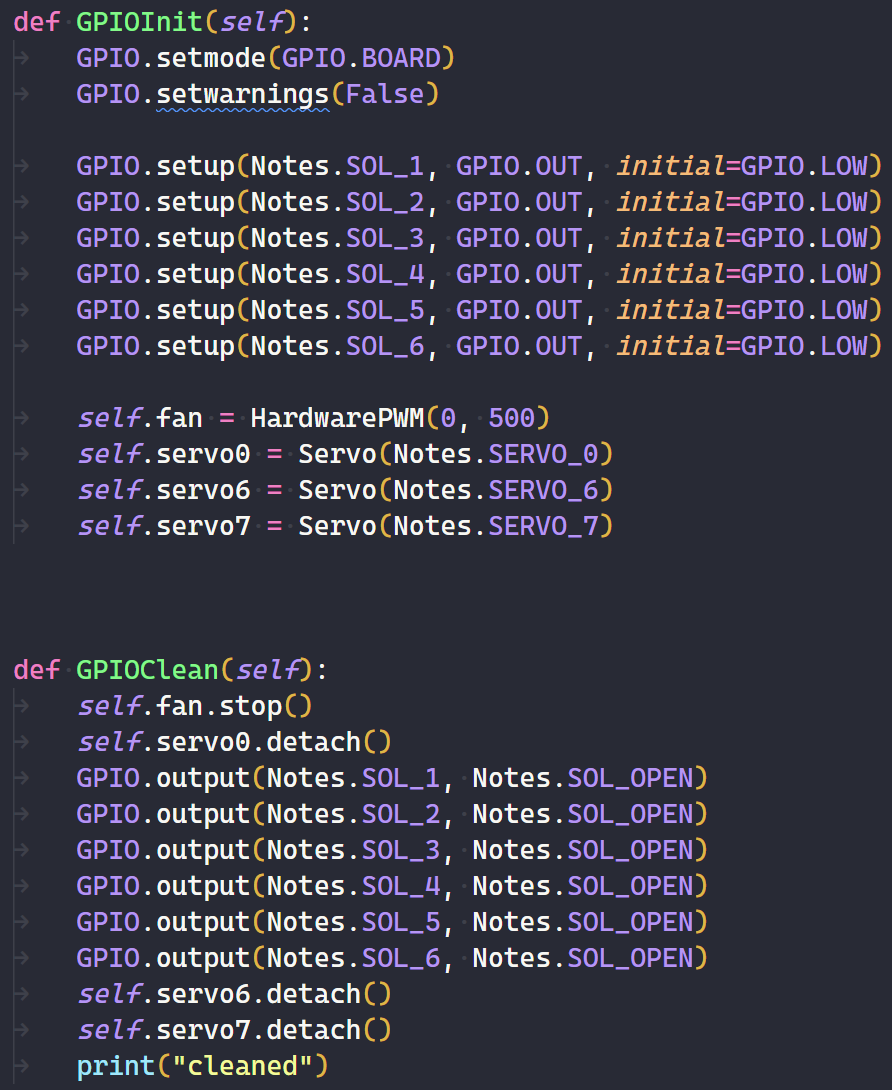
\includegraphics[width=0.75\textwidth]{gpio_init_code.png}
        \caption{GUI Setup Code}
        \label{gpio_init_fig}
    \end{figure}
    When any song or piano is active, the fan is started for a few seconds before the actual input begins playing, as the fan needs time to be able to push air at a usable rate. When a song is playing, the notes are played using a function which actuates all necessary solenoids and rotates servos, while altering the speed of the fan as required. This function is showed in Figure \ref{gpio_play_fig}.
    \begin{figure}[h]
        \centering
        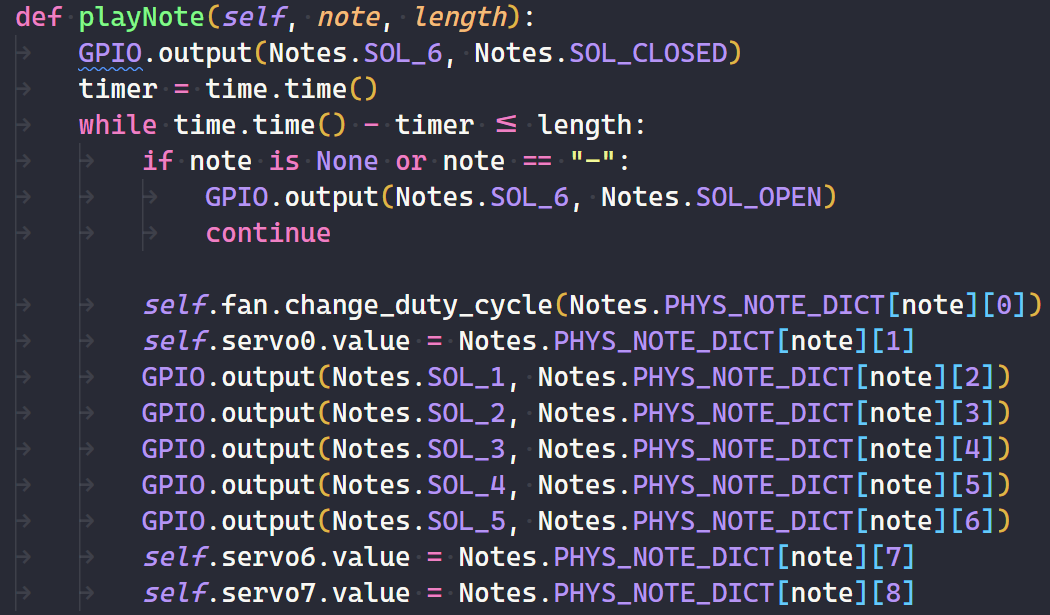
\includegraphics[width=0.75\textwidth]{gpio_play.png}
        \caption{GPIO Playback Code}
        \label{gpio_play_fig}
    \end{figure}

\subsubsection{Hardcoded Song Playback}
    As the main goal of the project is to be able to play a given list of songs, it was found that it was easier and more reliable to simply hardcode the songs that were needed. This is contained within the HardcodedSong class, shown in Figure \ref{hardcode_fig}.
    \begin{figure}[h]
        \centering
        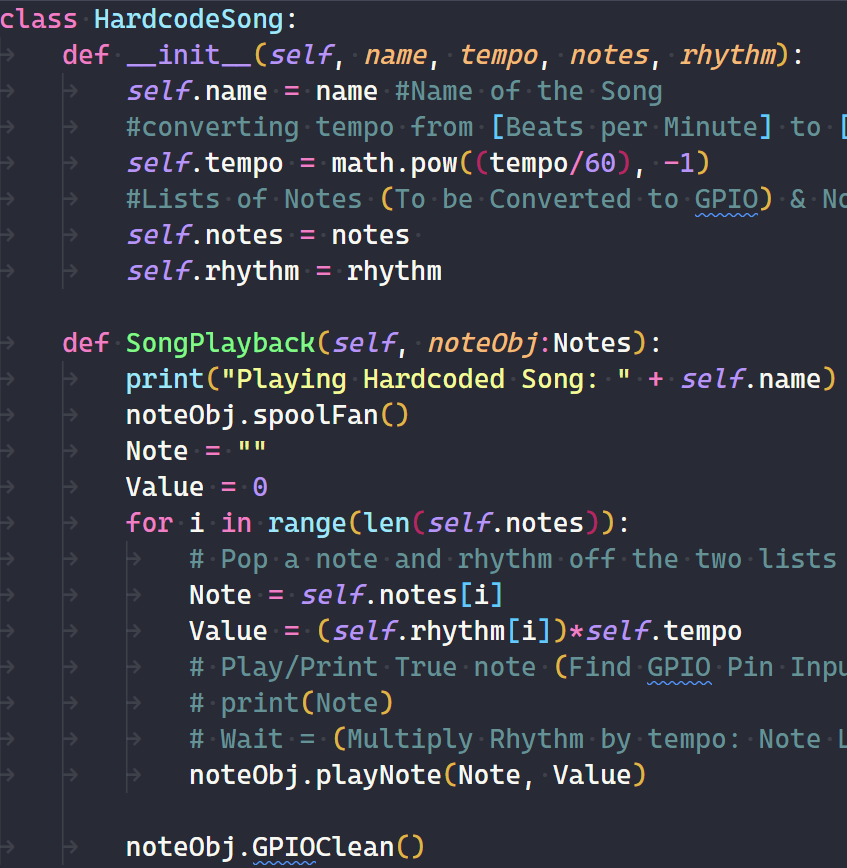
\includegraphics[width=0.75\textwidth]{hardcode_class.png}
        \caption{Harcoded Song Class}
        \label{hardcode_fig}
    \end{figure}
    \begin{figure}[h]
        \centering
        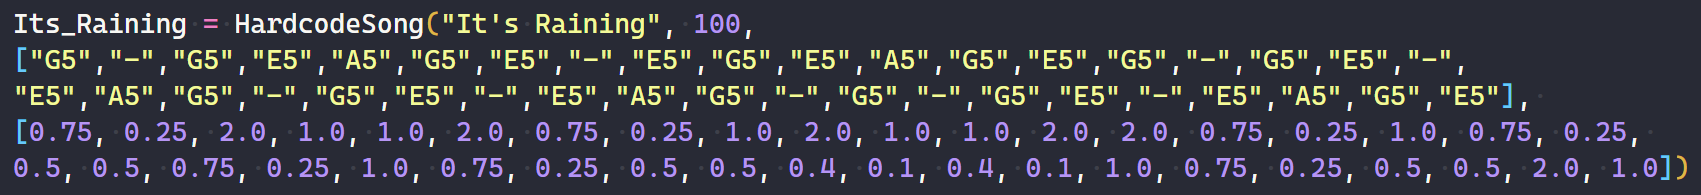
\includegraphics[width=0.75\textwidth]{hardcode_example.png}
        \caption{Harcoded Song Example}
        \label{hardcode_ex_fig}
    \end{figure}
    Figure \ref{hardcode_ex_fig} shows an example of how the class input is setup. The name of the song is first, then the tempo, then a list of the notes, then finally the list of timings. To play the song, the method SongPlayback is called on the instance. This loops through each of the notes and plays them for the allotted time, using the note playing class mentioned above.
\subsubsection{Custom Song Playback}
    To facilitate the playing of custom songs, a tab is there which consists of two buttons, a search for file button and a play button. The user first picks the MP3 file to play, then clicks the play song button to initiate the process. The bulk of the MP3 ingestion is performed by the software \textbf{ffmpeg}, originally developed by Fabrice Bellard and Bobby Bingham on December 20, 2000 \cite{ffmpeg}. 
    \begin{figure}[h]
        \centering
        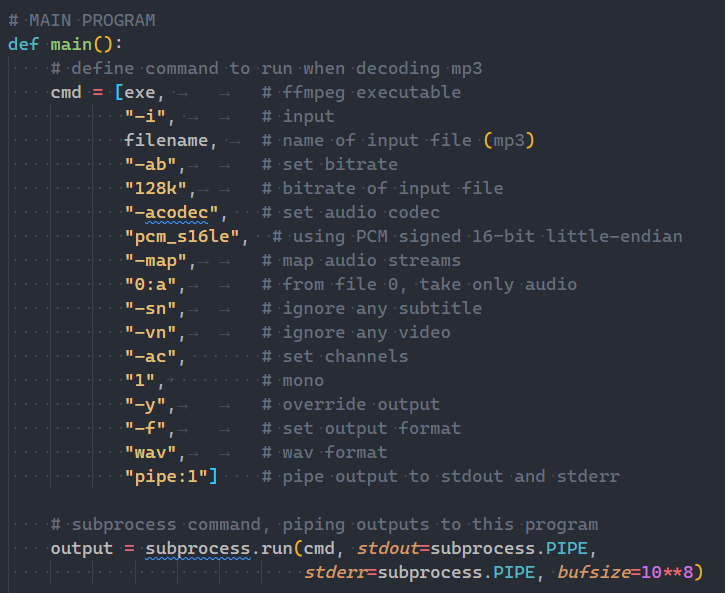
\includegraphics[width=0.75\textwidth]{ffmpeg_code}
        \caption{ffmpeg Command and Output Implementation}
        \label{ff_code}
    \end{figure}
    Shown in Figure \ref{ff_code}, certain command flags must be used upon executing the program in order to ensure proper output \cite{ffmpeg}. Some of the commands are less important, such as "-sn", which ignores subtitles or "-vn", which ignores any video streams (although this does implicate the software could feasibly process video data). Other commands are a necessity for proper output, such as "-f" and "wav", which sets the output format to a WAV file, and "-acodec" and "pcm\_s16le", which sets the output codec correctly. The most important flag there is "pipe:1" which outputs the WAV bytestream to the stdout, instead of dumping the output to a file. All of the output is contained in the variable conveniently named "output." Output consists of two properties, stderr and stdout. As stated above, stdout contains the bytestream of the output, but for debugging purposes stderr is useful as it contains the output of the command.

\subsubsection{WAV Parsing and Processing}
    Now that a WAV "file" has been obtained, work must be done in order to ascertain the correct values. The codec which was used to process the song is known as PCM, and the actual values that were output were unsigned 16-bit little-endian chunks. If one simply tried to read the bytes as they were, nothing but gibberish would be produced. This is because the bytes are little-endian, meaning the lower 8-bits are placed ahead of the upper 8-bits, effectively reversing the number in memory. As an example, take the decimal number \(2,500\). Its representation in a 16-bit hexadecimal is \(0x09C4\). Storing this value into contiguous memory locations would result in the following:
    \begin{equation*}
        0xC4 \to 0x09 \to ...
    \end{equation*}
    Attempting to get this value by only reading from left to right would return the number \(0xC409\), which is the decimal number \(50,185\), the incorrect value.

    To combat this, the Python package struct is used, as the programmer can tell the struct unpacking object what format to retrieve the bytestream as. This is done using format strings, in this case the string "<L". The < symbol tells the object the bytes will be little-endian, and the L tells the object to pack them into a 4-byte number \cite{struct}. This initial reading of the file allows the program to find the necessary sections of the file to read from.

    WAV files consist of a standardized structure \cite{wav}. They begin with a 44-76 byte header, depending on the WAV file creator. The program parses this header to either find the "fmt" section or the "data" section. The "fmt" section contains useful file information, such as number of channels, sample rate, and codec type. The "data" section contains, quite simply, all the actual song data. The program parses the "fmt" section for the information it needs to later process the "data" section. This is shown in below in Figure \ref{wav_code}.
    \begin{figure}[h!]
        \centering
        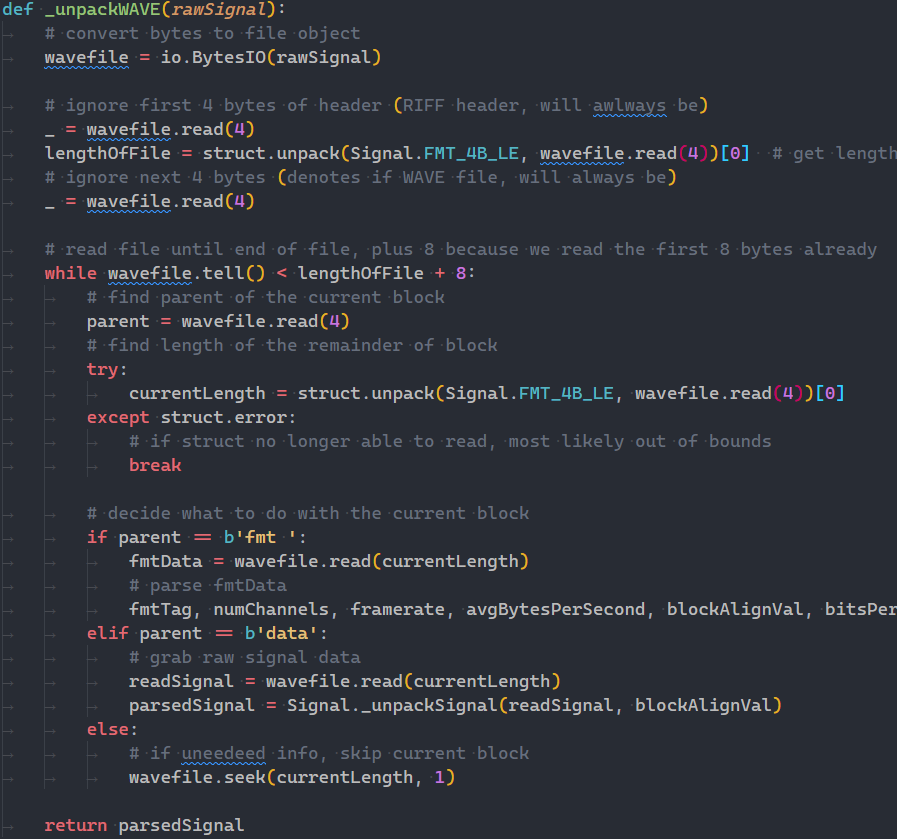
\includegraphics[width=0.55\textwidth]{wave_parse}
        \caption{WAV Processing Code}
        \label{wav_code}
    \end{figure}
    After this is complete, the variable "parsedSignal" is returned to the main program, which contains the actual waveform, and is then ready for further processing.

\subsubsection{The Fast Fourier Transform}
    While the program now has a long list of numbers which correspond to the waveform, shown below, the waveform itself is not a very useful signal for note processing.
    \begin{figure}[h]
        \centering
        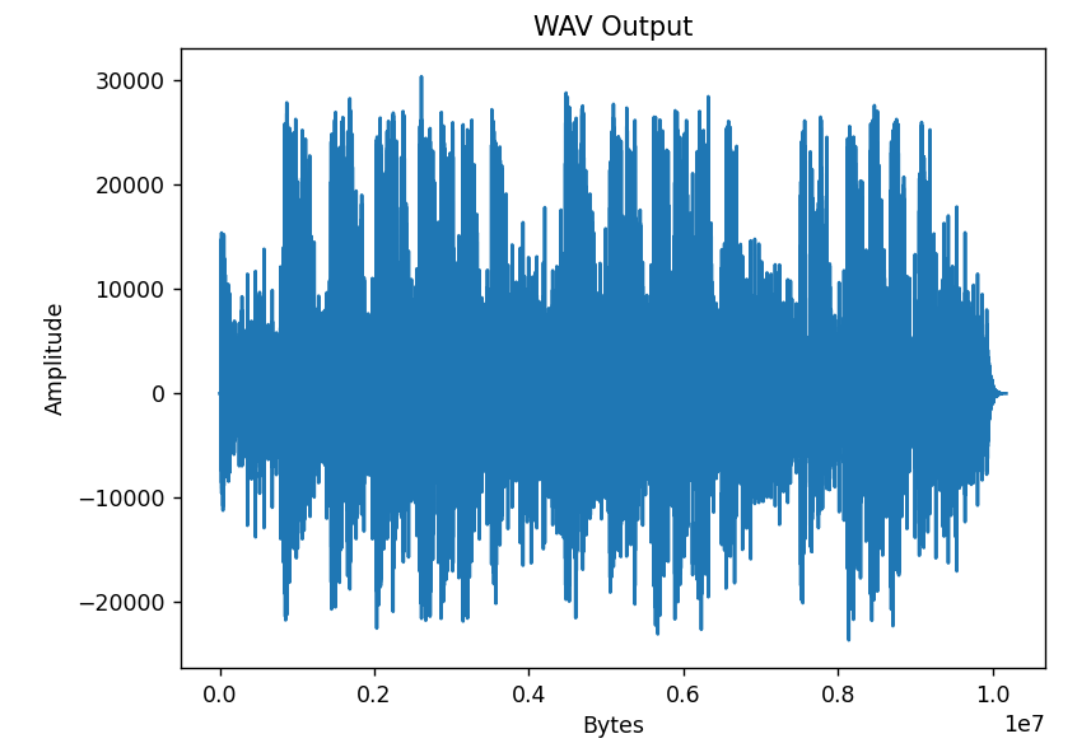
\includegraphics[width=0.75\textwidth]{waveform.png}
        \caption{An Example Waveform of a Song}
    \end{figure}
    These numbers are just the amplitude of the sound at that point in time, but to find the note at that point in time, the Fourier transform of the signal must be taken. The algorithm that has been implemented for live music processing is the Cooley-Tukey Fast Fourier Transform. This algorithm was popularized in 1965 by James Cooley of IBM and John Tukey of Princeton, although the original implementation was found to have been discovered in 1805 by Carl Friedrich Gauss \cite{fft_wiki}. The main premise is to recursively divide the Fourier transform into smaller and smaller chunks, which are then added back together at the end to produce the output \cite{fft_paper}. The standard Discrete Fourier Transform is defined by the equation \cite{fft_wiki}:
    \begin{equation}
        X_k = \sum_{n=0}^{N-1}x_ne^{-j2{\pi}kn/N} \quad k = 0 \; .. \; N - 1
    \end{equation}
    which is an $O(n^2)$ operation. The radix-2 algorithm brings this down to only $O(n\log{}n)$ through the recursion and division of the problem, leading to massive time and memory savings down the line. In order to save even more time for the sake of presentation, the original bytestream is sent over the network to a server which will then perform the FFT algorithm on the far more powerful Intel Xeon processors. The code is placed in a Docker container, which is a virtual machine inside of the server that can be enabled on input of the bytestream. 

    A prerequisite of this operation is that the provided signal must be a power of 2, which is where the time savings come from \cite{fft_wiki}. In order to this, the length of the signal is checked using the code in Figure \ref{check2_fig}, which compares the bits of the number and the number minus one. If the number is a power of 2, the result of ANDing them together would be 0, otherwise it would be any other number.
    \begin{figure}[h]
        \centering
        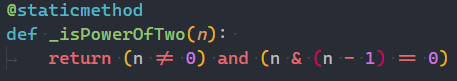
\includegraphics[width=0.75\textwidth]{check2.png}
        \caption{Function to Calculate if Number is a Power of 2}
        \label{check2_fig}
    \end{figure}
    Because the sample rate of the songs is 44.1kHz, and the windows of time are 100ms long, the number is not a power of 2, therefore the next highest power of 2 must be found and the signal must be extended to the new number.

    To find the next power of 2, a function which forces all the bits of the number to roll over until they are all 1's, then adds one to the number is used to calculate the next number to pad to. This is shown in Figure \ref{calc2_fig}.
    \begin{figure}[h!]
        \centering
        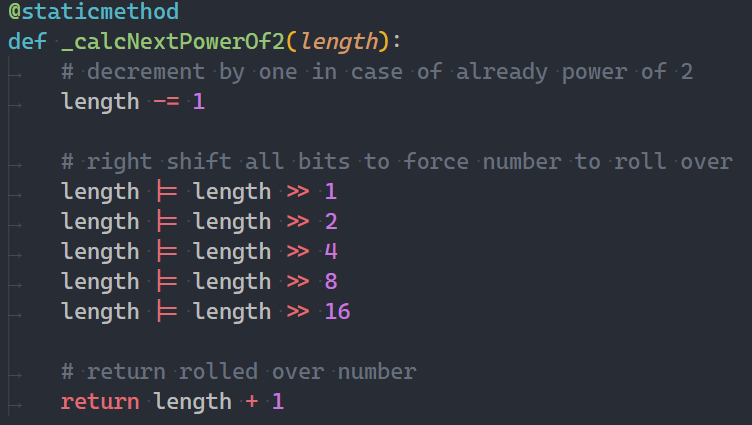
\includegraphics[width=0.7\textwidth]{calc2.png}
        \caption{Function to Find the Next Highest Power of Two}
        \label{calc2_fig}
    \end{figure}
    Once the signal is appropriately padded, the actual math can begin. The main algorithm consists of five steps:
    \newpage
    \begin{enumerate}
        \item Find the length of the current input list. If the length is one, return the list as is, otherwise continue.
        \item Using the length of the list, calculate $\omega$ using the formula $\omega = e^{j2\pi/N}$ where $N$ is the length.
        \item Break the current list into its odd and even elements.
        \item Pass the two new lists recursively into function.
        \item When the lists return, recombine the odd and even lists into a single list by raising $\omega$ to the current index of the loop and doing some other math.
    \end{enumerate}
    After these steps are completed the Fast Fourier Transform of the current list is complete.

\subsubsection{FFT Post-Processing}
    Once the waveform is converted from a time domain signal into a frequency domain signal, further work must be done to transform the current values into usable frequencies. To do this, the highest magnitudes of the bins of values must be calculated. First, the second half of the signal is discarded, as the second half if just the complex conjugate of the first half \cite{fft_wiki}. Then, the absolute value at each point is taken, as this is a real signal, the imaginary and negative components are irrelevant. Finally, the actual magnitude is calculated. To do this, loop through the remainder of the list, and at each even and odd point treat the even as the real component and the odd as the imaginary, then combine them using the following formula:
    \begin{equation}
        Magnitude = \sqrt{Re^2 + Im^2}
    \end{equation}
    These magnitudes are then inserted into their own list, where the largest value corresponds to the highest peak in the frequency spectrum, which is almost always the frequency at that point in time. An example of the peaks is shown below in Figure \ref{peaks}.
    \begin{figure}[h]
        \centering
        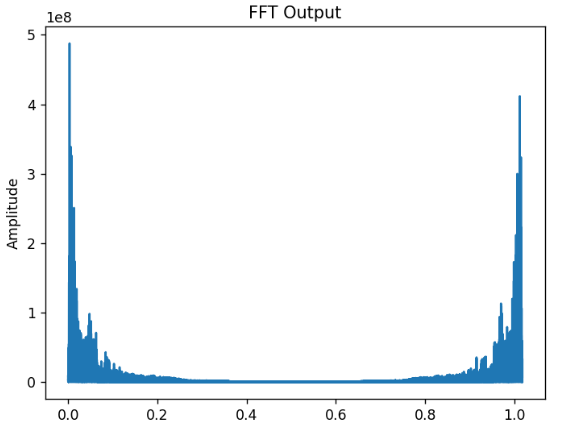
\includegraphics[width=0.75\textwidth]{fft_peaks.png}
        \caption{Example of the FFT Output}
        \label{peaks}
    \end{figure}
    To find the actual frequency associated with the peak, the equation as shown below can be used:
    \begin{equation}
        Frequency = \frac{(index\;of\;largest\;peak) * (sample\;rate)}{(length\;of\;bin)}  
    \end{equation}
    
    To actually play a song, the frequencies are placed into a list, where repeated frequencies are counted and divided by 10 to calculate the time required to play that note. To find the note, a $\pm$5 percent range is calculated around the frequency, which is used as a key for a dictionary with the frequencies to notes built in.

    Once those notes are found, those notes are rounded up and down into the actual playable notes on the recorder. This is done by comparing the note to a list of notes which the reorder can physically play. The note is then played for the length of time calculated before using the note playing method in the note class.
    
\subsubsection{Piano Input}
    To play the piano, another tab is included which consists of two buttons, a play piano button and a stop playing button. The stop playing button is required as the function, shown in Figure \ref{piano_play}, is permanently stuck in a loop which looks for input until a certain flag is marked true. To make sure the program is not locked up upon hitting the start playing button, the initial piano playing process is actually being run in a seperate thread, which is done by using the Python library threading, a library that leverages the CPU's multiple cores for concurrent parallel execution.
    \begin{figure}[h]
        \centering
        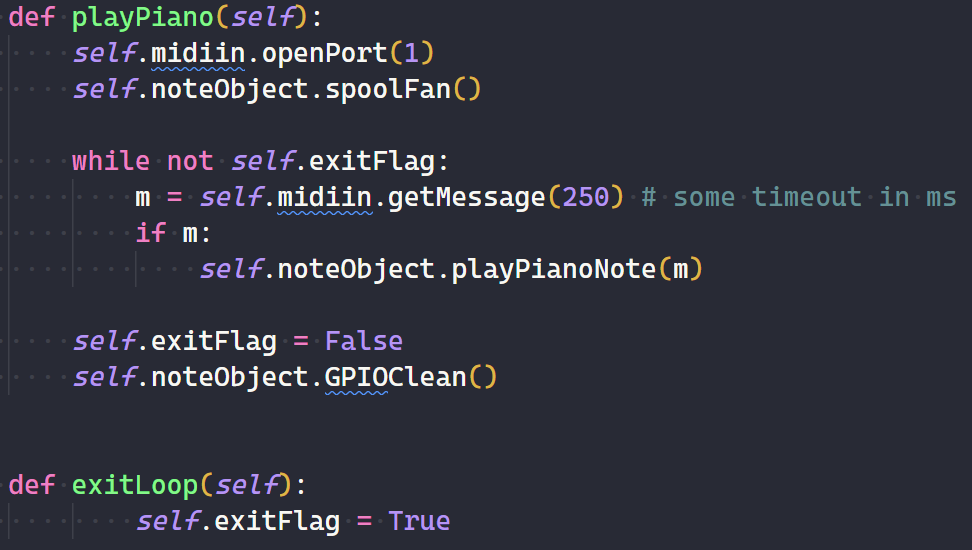
\includegraphics[width=0.75\textwidth]{piano_play.png}
        \caption{Piano Playing and Exit Functions}
        \label{piano_play}
    \end{figure}
    The exitLoop function is also executed in a separate thread as to not lock up the main thread which keeps the main thread free for other program usage.

\subsection{Hardware}
\subsubsection{The Recorder}
    As the main goal of the project is to play a recorder automatically, the most important facet of the hardware is the recorder itself. The YRS-24B is the instrument used. This recorder is fairly standard, and is tuned in C. Figure \ref{rec} depicts the recorder.
    \begin{figure}[h]
        \centering
        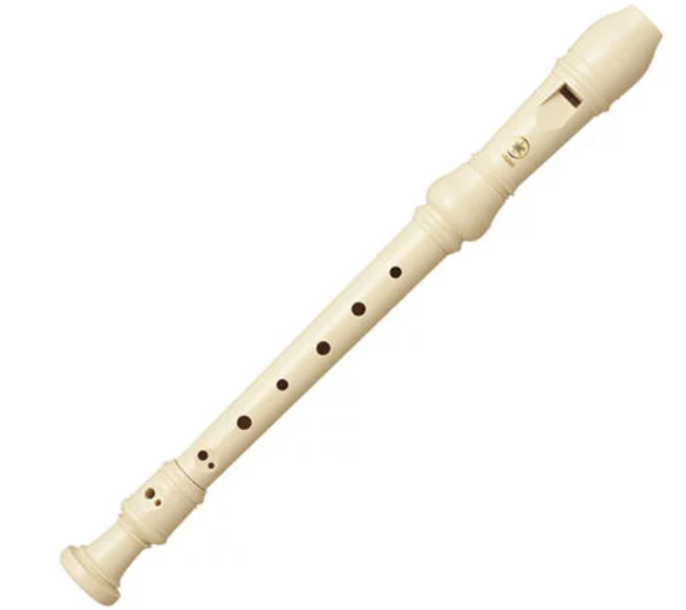
\includegraphics[width=0.75\textwidth]{recorder.png}
        \caption{The Yamaha YRS-24B Recorder}
        \label{rec}
    \end{figure}
    This specific recorder can play notes from C5 to D7, which is a range of 27 total notes. Playing is accomplished by blowing into the mouthpiece and covering and uncovering the holes as required by each note and octave. This recorder also has a rotating end piece, which makes it easier to articulate with rigid mechanical components, and is used to tune the instrument.
    \newpage
\subsubsection{Airflow}
    The recorder is a woodwind instrument \cite{rec_wiki}, and being so it requires airflow to play. The proper airflow requirement is around 0.1 to 1 liter per second \cite{rec_info}, therefore while the speed of the air is less important, generating the correct amount airflow is necessary for good sound. To produce a balance between too much and too little airflow, a single blower fans are mounted in series in order to control the flow. This is shown in Figure \ref{fan_fig}.
    \begin{figure}[h]
        \centering
        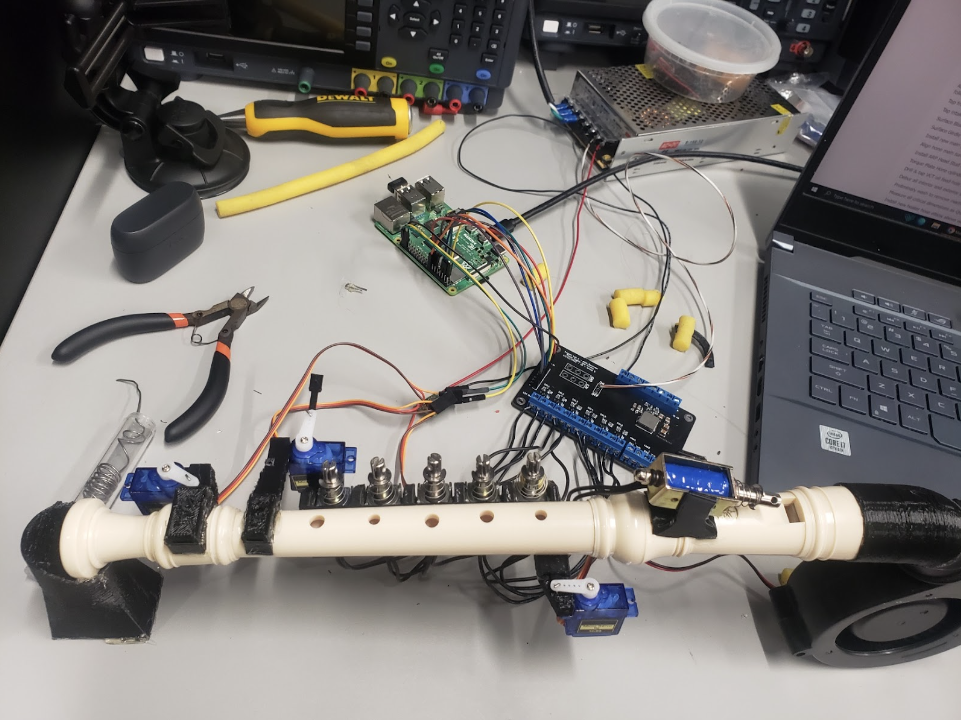
\includegraphics[width=0.75\textwidth]{recorder_fan.png}
        \caption{Recorder Fan Setup}
        \label{fan_fig}
    \end{figure}
    The fan is a Sparkfun 12V blower, a DC fan that can output 16CFM at 3500 RPM\cite{fan_info}. This blower motor provides the perfect amount of airflow and is simple to increase or decrease at will. Controlling the air is done through a hardware PWM port with the Raspberry Pi.

    \subsubsection{Solenoids and Servos}
    While the correct amount of air now properly flows through the recorder, only a single note would play if the holes are not used. To do this, a series of five solenoids and three servos is used. The five solenoids are meant to actuate the holes facing upwards, where a fully open or fully closed state is acceptable. For the holes that require variably closed and open states, the three servos are positioned under the recorder to close and open them as needed. A 3D model of the system is shown below in Figure \ref{rec_set_fig}.
    \begin{figure}[h]
        \centering
        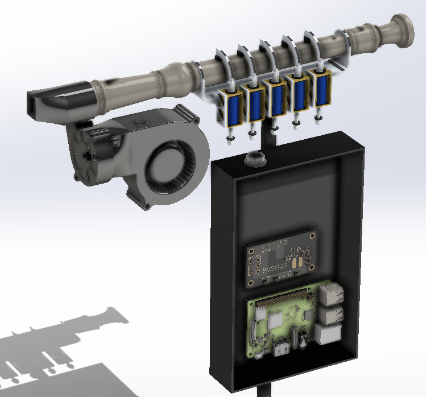
\includegraphics[width=0.75\textwidth]{rec_setup.png}
        \caption{3D Recorder Model}
        \label{rec_set_fig}
    \end{figure} 

    The solenoids are rated for 12V, 1A at around 500g of actuation force. In reality, that is closer to around 600mA, but everything designed is rated for 1A. As stated previously, the Pi can only output 5V at 16mA, so a circuit has been designed in order to drive them. The power supply, which will be discussed later, provides both 12V and 5V, so a MOSFET is activated with the 5V GPIO signal, which allows 12V power to run the solenoids. The solenoids are inductive loads, so when they are deactivated, a spike of current flows back into the circuit. To protect the main circuit, a flyback diode is used to stop the current. This is shown in Figure \ref{sol_ckt}.
    \begin{figure}[h]
        \centering
        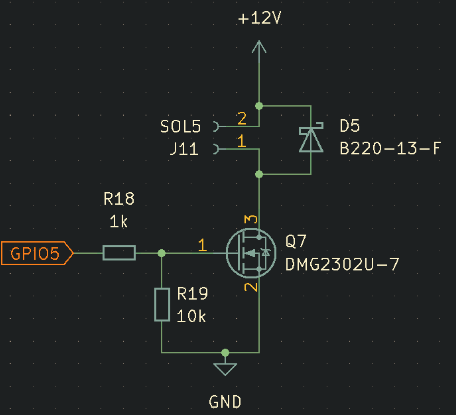
\includegraphics[width=0.75\textwidth]{solenoid_ckt.png}
        \caption{Solenoid Circuit Diagram}
        \label{sol_ckt}
    \end{figure}
    For the flyback diode, a Schottky diode is used for its fast switching abilities and high reverse breakdown voltage. When the GPIO pin is high, 12V flows through the circuit, which then can enter the solenoid. The servos are connected to dedicated 5V outputs, and the positions are controlled with the dedicated PWM connection.
    \subsubsection{Power Supply and Driver PCB}
    \begin{figure}[h]
        \centering
        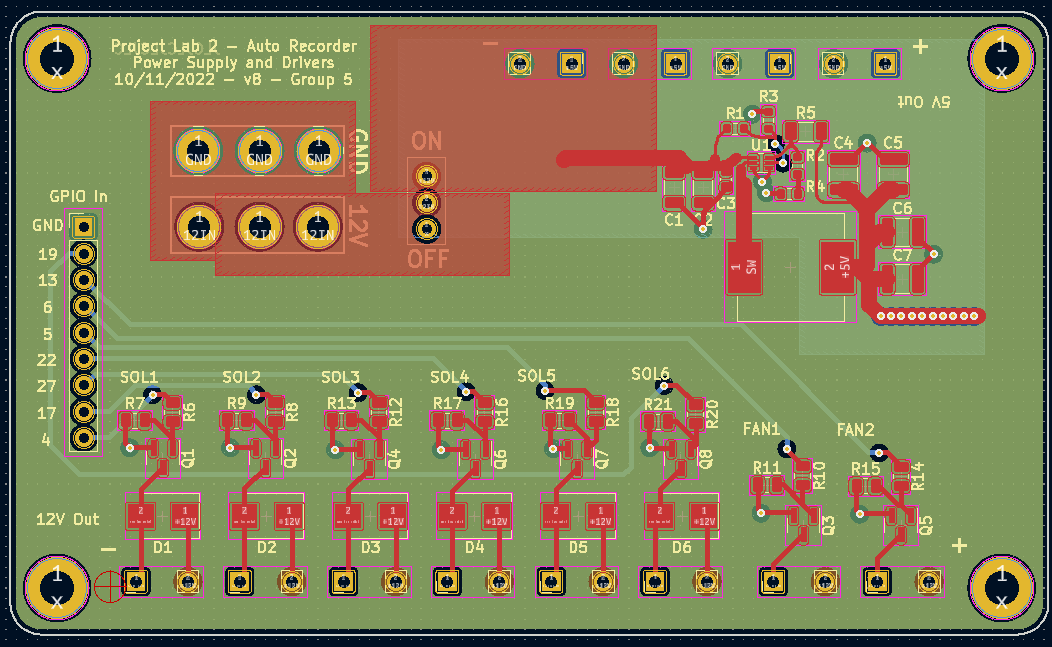
\includegraphics[width=0.75\textwidth]{pcb.png}
        \caption{Main PCB}
    \end{figure}
    The PCB has been designed to provide power and outputs for all connected hardware. It is capable of providing a maximum of 12V at 7A and 5V at 6A. Input power is provided from a 12V, 15A AC to DC power supply, and is connected to the board using a GX-16 6 pin connector. A switch connects this input to the rest of the board, which then sends the power to the rest of the board.

    The 5V is generated with a TPS566247DRLR, a 5V, 6A switch mode power supply. This voltage is output to four connectors, three for the servos and one for the Pi. The rest of the raw 12V power is routed to the six solenoid drivers and two fan drivers, which is the same circuit as the solenoid driver but lacking a flyback diode. The board is a four layer design, with a stackup consisting of signal-ground-12V-signal, measuring 1.6mm thick. The board is 100x60mm, with four M3 bolt holes for mounting to the apparatus. 

    \subsubsection{Computational Power}
    \begin{figure}[h]
        \centering
        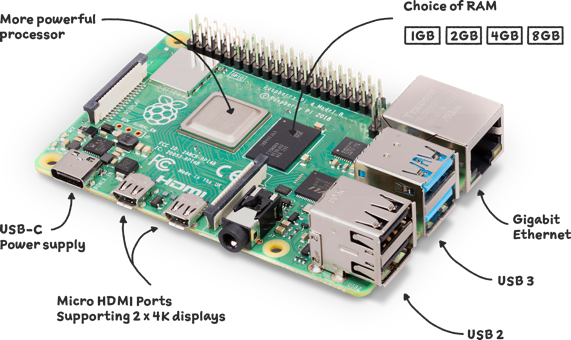
\includegraphics[width=0.65\textwidth]{rpi.png}
        \caption{The Raspberry Pi Model 4B}
    \end{figure}
    The Pi used is a 4GB model with a quad core ARM processor. To aid the speed of the FFT execution for songs, the process will be sent to another server over the internet and then multithreaded using Python's builtin threading library. GPIO pins 4, 17, 27, 22, 5, 6, 13, 19 are connected to the various solenoid and servo outputs. To provide the least overhead possible, instead of installing a full-fledged operating system, a headless version of Raspbian is used in combination with SSH for access.
\section{Conclusion}
    As of writing this paper, the project is complete and works well. The speed of the played songs is a little bit slower than the typical way one might sing the songs, that is not an issue of the device itself, its just the rhythm of the song as was programmed. The final touch before presenting to the elementary school we will be at is putting all the parts inside of a case to neatly tie everything up. The project went smoothly, and although there were a few changes in between the midterm paper and now, there were no significant pivots to other technologies. 

% \newpage
\section{Appendix}
\subsection{GANTT Chart and Budget}
    \begin{figure}[h]
        \centering
        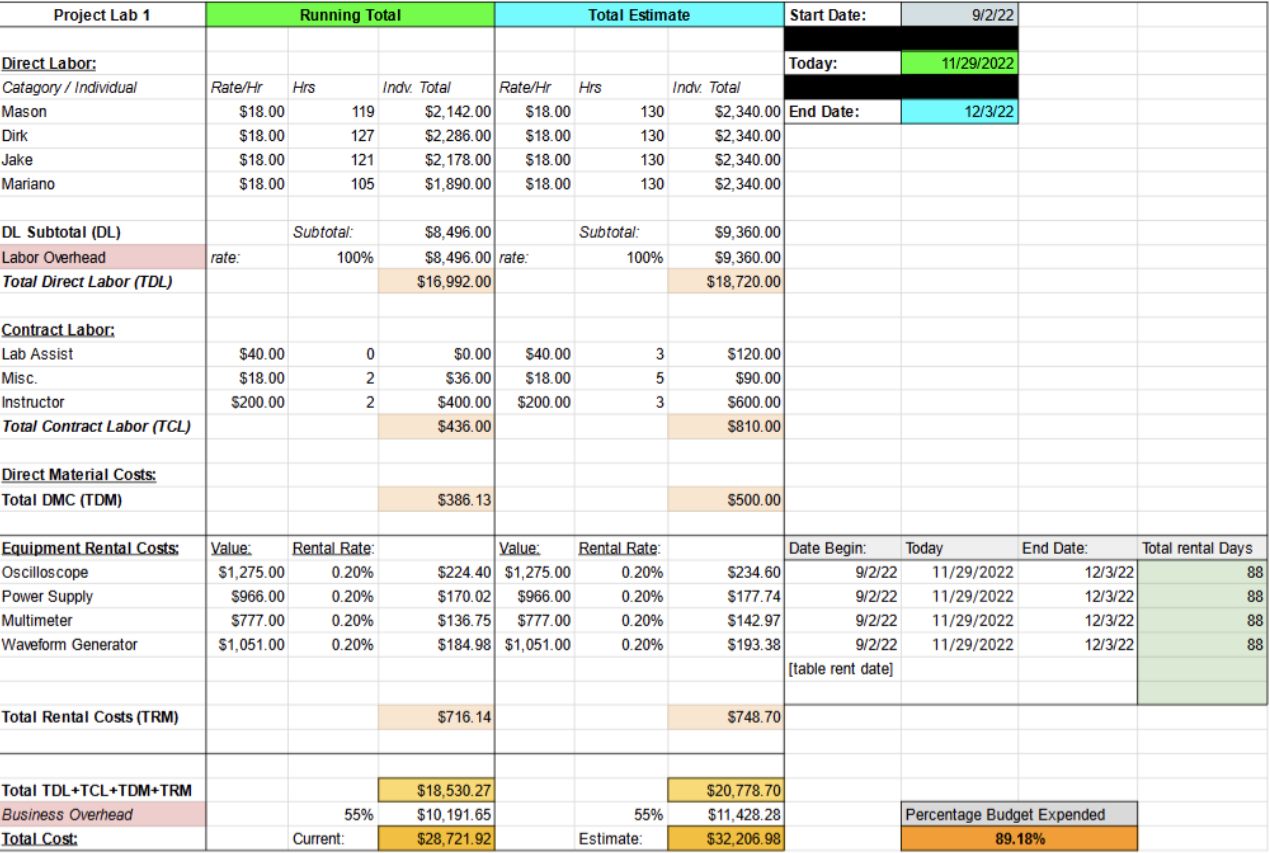
\includegraphics[width=0.75\textwidth]{budget.png}
        \caption{Current Budget}
        \label{bud_fig}
    \end{figure}
    \begin{figure}[h]
        \centering
        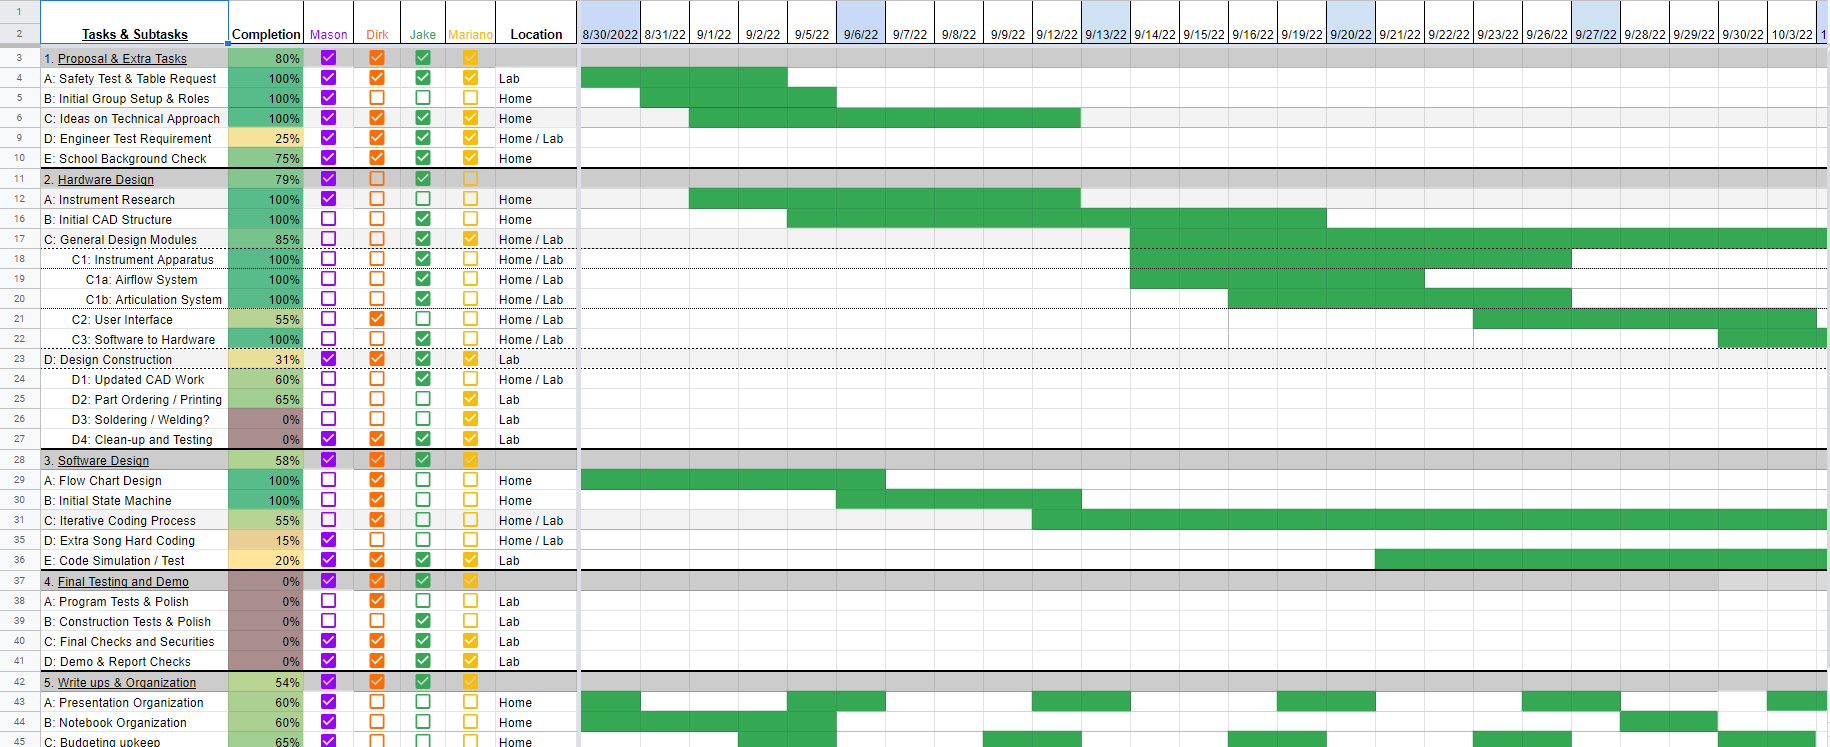
\includegraphics[width=0.75\textwidth]{gantt.png}
        \caption{Current GANTT Chart Progress}
        \label{gan_fig}
    \end{figure}
    As shown in Figures \ref{bud_fig} and \ref{gan_fig},the budget and GANTT progressed perfectly on schedule and under budget. The final budget total was around 89\%, which shows that the total amount was calculated correctly. The GANTT chart is completely satisfied as well.
\subsection{Safety and Ethics}
    Special considerations must be thought of safety wise, as this project is meant to be presented to a classroom of elementary schoolers. Because of this, care has been taken to ensure AC power is never exposed anywhere a student might touch, and that the touchscreen access in general should only be relegated to the teacher of the classroom or the people of the lab group. It is also important to consider volume levels, as overblowing the recorder could cause a loud, sharp noise which could hurt a student. The maximum airflow of the fans has been found, and it is within an acceptable range as to not hurt any hearing. The ethical ramifications stem from the fact that human musicians are already paid very little for their talents, so developing an automated system to play an instrument might lead to less jobs. However, this machine will never be able to be as versatile and talented as a real person playing, so I think it is safe to say this shouldn't hurt any chances.

\newpage
\printbibliography

\end{document}